% TODO: maybe add another section about how vectorization actually works in archetypes vs types?

\section{Concurrency Model}
\label{chap:2}
The following chapter introduces a formal concurrency model written of this paper's own design. The core of the paper is the theory proposed here. The GECS Library uses this theory to orchestrate components to ensure an acceptable degree of wait-free concurrency. This concurrency model is of this paper's own design. It's inspired by FLECS in the way that it vectorizes type compositions.

\subsection{Formal definition} \label{section:formal_definition}
We define the following called a world context to be a property that exists in an ECS: $W = (T, A, \delta, \Lambda)$ consisting of:
\begin{enumerate}
    \item A finite set of types $T$.
    \item A set of archetypes $A \subseteq \mathcal{P}(T)$, where $\mathcal{P}(T)$ denotes the power set of $T$.
    \item Some transition function $\delta : A \times T \rightarrow A$.
    \item A set of systems $(\lambda, \lambda_{req}) \in \Lambda$ such that $\lambda : W \rightarrow W^\prime$ and $\lambda_{req} \subseteq \mathcal{P}(T)$ representing the types required to initiate $\lambda$.
\end{enumerate}

\subsubsection{World Contexts}
$W$ represents the concept of a world, or one simulation, within the ECS. The ECS ensures that the following properties in context to worlds hold:

\begin{enumerate}
    \item An ECS may contain multiple worlds, but must have at least one.
    \item Only one world can be considered to be the "real" context.
    \item All worlds except one can be considered to be in the "simulation" context.
\end{enumerate}

At a very high level, the real context contains all vectorized data and the simulation context contains future operations to be applied to the real context that are not able to be done concurrently. Later in this chapter, the paper provides a proof as to why certain operations within this concurrency model cannot be done in parallel. 

This definition will later be used in this chapter to generate the entity finite-state-machine (FSM).

\subsubsection{Systems}
Systems are a tuple containing two properties: $\lambda$ and $\lambda_{req}$. $\lambda_{req}$ is a set of types that can be used to match $\lambda$ to archetypes. All archetypes that are super-sets to $\lambda_{req}$ get matched with an archetype.

The second part to systems is the $\lambda$ function. This function takes in a world context, either the real context or a simulated one, and applies a set of mutations and returns a copy. This altered copy is then used to merge all entity FSM's into the real context after some serialization point in the future.

\subsection{Types And Archetypes Relationships}
Until now, components were assumed to be stored in large, homogeneous vectors. This is great for cache locality, vectorizability, and is optimal for an ECS. But such a system when put in a runtime environment quickly falls apart, namely when composite type entities are introduced (entities with more than one component). 

Where should new entities get placed? In vector A or vector B? If the vectors are forced to be homogeneous, and an entity is included that only has A xor B, then the length of A and B are different. This is not ideal for SIMD, so we want to introduce a system that allows for the existence of composite entities, without losing out on vectorized operations.

Archetypes are a composition of types that exist within $\mathcal{P}(T)$. Archetypes, argued later in this chapter, are always able to maintain their vectorizability. Archetypes are critical for this concurrency model to work. They are the foundation on which what is able to be parallelized during the GECS runtime \cite{SanderMertensECS}.

\subsubsection{The ABC Problem}

The ABC Problem is a problem introduced by the FLECS creator Sander Mertens \cite{SanderMertensECS}. The problem demonstrates the effectiveness of Archetypes in component storage while retaining its vectorizability property -- and it's a good introduction to archetypes.

Suppose there exists a set of entities $E$ and $n = |E|$. Suppose $T := \{A,B,C\}$ and for each type $t \in T$, there exists a homogeneous vector containing elements of type $t$. Then, if all entities in $E$ have all components this is the following layout of the ECS in memory:

\begin{figure}[H]
    \begin{lstlisting}[
        language=Java,
        numbers=none
    ]
    A components[n];
    B components[n];
    C components[n];
    \end{lstlisting}
    \caption{Homogeneous ECS Components}
    \label{code:homogenous_ecs}
\end{figure}

In this ideal world, entity ID's can be emulated by simply being the index to the vectors. This is possible because the indexing property for this scenario $\forall t \in T : |t| = n$ holds. This ECS is positioned advantageously because all vectors are contiguous and therefore are vectorizable. This is only true because of the indexing property mentioned.

Suppose during runtime one of the entities at some index $k$ removes some component $t$. In such a situation, the defined indexing property is broken because not all vectors are of the same length and the gap in memory now means vector operations will be slow.

Sander Mertens uses this setup to prove that an ECS cannot vectorize homogeneous components efficiently at all. This is done by reviewing all situations in which homogeneous components are mutated to make vectorization impossible or difficult. By the end, he presents an elegant alternative called archetypes and proves that archetypes leads to some form of good vectorizability.

\subsubsection{Archetypes}
Simply put, an archetype is a set of types. Archetypes add a layer of abstraction on top of types so to make ECS queries vectorizable. Instead of creating homogeneous vectors based on types in $T$, we can create homogeneous vectors based on archetypes in $A$. 

\begin{figure}[H]
    \begin{lstlisting}[
        language=C
    ]
    A a[A_len];    /* Archetype {A} Part: "A" */

    A a[AB_len];   /* Archetype {A,B} Part: "A" */
    B b[AB_len];   /* Archetype {A,B} Part: "B" */

    A a[AC_len];   /* Archetype {A,C} Part: "A" */
    C c[AC_len];   /* Archetype {A,C} Part: "C" */
    \end{lstlisting}
    \caption{ECS Components With Archetypes $\{\{A\},\{A,B\},\{A,C\}\}$}
    \label{code:ecs_archetypes}
\end{figure}

Even though in Figure \ref{code:ecs_archetypes} those arrays are independent they do not have to be. In the GECS implementation, for example, all components of an archetype are interleaved into a contiguous array. So archetype storage looks more like that of Figure \ref{code:homogenous_ecs} than Figure \ref{code:ecs_archetypes}. Figure \ref{fig:composite} elaborates on what is meant by interleaved components. This is called the composite.


\begin{figure}[htbp]
    \centering
    \begin{verbatim}
Archetype X:                                                             
+---------+---------+-------------+---------+---------+-------------+---+
|Component|Component|Component    |Component|Component|Component    |   |
|A      8B|B      8B|C         16B|A      8B|B      8B|C         16B|...|
+---------+---------+-------------+---------+---------+-------------+---+
    \end{verbatim}
    \caption{Example Composite Vector Of Archetype X}
    \label{fig:composite}
\end{figure}

The composite vector can contain components of varying lengths. Component C is twice as large as Components A and B. Note that since archetypes are sets of types, archetypes $AB \equiv BA$ represent the same archetype.

\subsection{Representing Archetypes As An Entity Finite-State-Machine}
\label{sec:fsm_arc}
ECS applications are expected to handle operations over entities that can add, modify, or remove components. In the context of archetypes, this means being able to transition an entity between them. 

An example of such a situation is a game. Suppose all entities within the proximity of some point in space gain a tag component saying "buffed", but when they leave the proximity the tag component is removed. These types of state transitions may occur hundreds of times and need to be performant. 

\subsubsection{The Entity FSM}

A finite state machine emerges from using archetypes to organize entities in a specific way. If the addition and removal of components are considered as state transitions, then the following in Figure \ref{fig:graph1} represents existing archetypes during some ECS runtime. We define vertices to be archetypes in $W$ and edges to be entity transitions to adjacent archetypes.

As an example, suppose we have an ECS with the following properties:
\begin{align}
    T &= \{A,B,C,D\} \\
    A &= \{ \emptyset, [A] , [A,C] ,[B], [A,B], [A,B,C], [B,D], [D]\} \\
    \Lambda &= \emptyset
\end{align}
                                    
\begin{figure}[htbp]
    \centering
    \begin{verbatim}
                      +---------+       +---------+                                  
        +------------>+   [A]   |<----->|  [A,C]  |<--------+                        
        |             +---------+       +---------+         |                        
        v                                    ^              v                        
   +---------+        +---------+            |         +---------+                   
   |   [ ]   |<------>|   [B]   | <----------+         | [A,B,C] |                   
   +---------+        +---------+                      +---------+                   
        ^                  ^  ^                             ^                        
        |      +---------+ |  |          +---------+        |                        
        +----->|   [D]   | |  +--------->|  [A,B]  +--------+                        
               +---------+ |             +---------+                                 
                           |  +---------+                                            
                           +->|  [B,D]  |                                            
                              +---------+                                            
    \end{verbatim}
    \caption{Example FSM Graph Of Archetypes During Runtime}
    \label{fig:graph1}
\end{figure}

As shown in Figure \ref{fig:graph1}, all graphs contain the empty set $\emptyset$ as a vertex. This is because all entities when initiated contain the archetype with no components. As components get added to entities over their runtime, entities perform state transitions to their designated archetype.

It's important to remember that a serialization point is when the tick increments. All state transitions and entity states before the serialization point are considered invalid. Because of this, we know that entities require only one real transition per tick to a valid state. 

This means an entity could perform the transition, say $\{B,D\} \rightarrow \{A,B,C\}$ in one step, even though it passes through archetypes $[\{B\}, \{A,B\}]$ on the FSM. On the next tick, the edge $\{B,D\} \rightarrow \{A,B,C\}$ will be present. 

Entity Finite State Machines display the following properties:

\begin{enumerate}
    \item All existing archetypes must have a path to vertex $\emptyset$.
    \item Components can appear multiple times.
    \item Archetypes can only appear once.
    \item Entities can only appear once at one archetype.
\end{enumerate}

There are a couple interesting things to notice in Figure \ref{fig:graph1}. Notice how there is no transition between state $[B,D]$ and $[D]$. This is because this graph represents a runtime of an ECS and while it is possible to transition between $[B,D] \leftrightarrow [D]$, it has yet to happen in this runtime context, and is therefore not required to exist. 

The component $C$ in Figure \ref{fig:graph1} is special in the regard that it is not adjacent to the $\emptyset$ vertex like the others. This does not mean that it is impossible to create an entity with only component $C$ but that the runtime has yet to have that situation occur.

To loop back to the proximity example in the introduction in section \ref{sec:fsm_arc}, by representing additions and deletions as runtime state transitions it should now be clear that large performance gains are achieved via these edges. Initially, the first entity that transitions between two states in the simulation will be slow because the edge between those two vertices must be made. Once that edge is made, it is cached and the deletion and transfer of an entity to another archetype drops from $O(N)$ to $O(1)$.

\subsubsection{Operations On Entity FSM}
The following operations are all thread safe due to the scheduling algorithm explained in section \ref{sec:scheduling}. All implementation details are abstracted away except the operations directly done on the FSM. 

\textbf{Entity Creation:} All entities when created start at the $\emptyset$ vertex. All entities that exist here are not query-able.

\textbf{Entity Component Addition/Deletion:} Aside from the simple transition using an existing edge. When a component addition occurs, two operations are completed. Suppose the archetype we are currently in is at archetype $G$ and are attempting to add component $C$. This mean we are attempting to transition to archetype $G \cup \{C\}$. The two operations required for component addition are lookup and connection operation.

\begin{enumerate}
    \item If $G \cup \{C\} \not\in A$, then do step 2. Else do step 3.
    \item Create a new archetype $G \cup \{C\} \in A$. Apply component addition.
    \item Create the edge $G \leftrightarrow G \cup \{C\}$. Apply component addition.
\end{enumerate}

Both component addition and deletion use the same transition function $\delta$, so the component deletion operation is the same procedure.  

\textbf{Entity Deletion:} When an entity is marked for deletion, the archetype has the choice to either delete it now or wait to delete all entities together in a batch at some point in the future. Both of these strategies are thread safe. 

What happens when an archetype loses all its entities? While it would make sense for the archetype to be deleted from the graph since no entities are there, and it'll keep it mathematically pretty, there's not much theoretical reason as to why they should be kept. 

In practice though, there's a decently high probability that archetype will gain an entity again. Deleting those edges to archetypes with no entities will only slow down specific entity transition patterns. The memory usage of an empty archetype is also inconsequential and so there is no real trade-off of keeping it alive.

\subsection{Scheduling Systems}
\label{sec:scheduling}

Due to the nature that ECS follows principles in data-oriented design, these architectures have an advantage in concurrency contexts. The following section is about an algorithm designed in this paper to schedule systems concurrently in such a way they produce one valid serialization point per tick. Therefore, this algorithm does not guarantee that all entities will enter a system in any order or be processed in some order. Entities may be sent to the system seemingly at random.

\subsubsection{Scheduling Algorithm}
Before discussing the scheduling algorithm, we must define more strictly what functions are allowed to query in this architecture. Since archetypes and the state machine are abstracted away from the user, the set of rules for what is query-able and what is not should not be exposed to the user. The architecture must handle all query requests and attempt to parallelize as much as possible. 

Generally, if there exists an archetype that is the super-set of the query, then the query is OK. But asking a library user to only query in sets of existing archetypes is unreasonable. If the user, for example, in their render system wants to collect non-associated components \texttt{[Position, Score, Health]}, the ECS will fail. There is no archetype that holds these three random components together. This would make the query a super-set of archetypes and this use case must be handled in some manner that keeps the concurrency model valid. 

The way this scheduling algorithm solves this is by asking the user to always give the intersection of required types. For this example, suppose:
\begin{itemize}
    \item Player contains \texttt{[Position, Texture, Inputs, Health, Score]}
    \item Enemy contains \texttt{[Position, Texture, Health, Bullets Left]}
    \item Game Objects contain \texttt{[Position, Texture]}
\end{itemize}

The intersection between (Player $\cap$ Enemy $\cap$ Game Objects) is a \{\texttt{Position, Texture}\} component set. Therefore the render system should request only for the those two components. This will allow the ECS to correctly queue up each of those entities as concurrently as possible. 

But what about the other data? If I only query for \texttt{Position} and \texttt{Texture}, how will I access \texttt{Score} and \texttt{Health}? By applying the 4th property of the entity FSM: entities can only appear once at one archetype, we know that only one version of the entity can exist at one time. It is actually safe to load the rest of the entity data off the archetype when its time to process a queried entity. This is because we are guaranteed to be the only ones who have access to this entity at a given time. Any component that is hidden only needs to have their entity tested to see if that component is available for that entity.

With this in mind, the only function class allowed to be given to the scheduling algorithm from the user are functions whose requirements are a subset or equal to some archetype type set in $A$. The archetype concept can be blanketed away from the user by requesting all queries to contain the minimal intersection of types. The simple algorithm below assigns each function on the Entity FSM as such:

\begin{figure}[H]
    \begin{enumerate}
        \item For each $\lambda \in \Lambda$, do the following steps 2-3:
        \item Construct the set $x = \{\forall a \in A : \lambda_{req} \subseteq a \} \setminus \{\emptyset\}$.
        \item For each archetype in set $x$, mark that archetype to run $\lambda$.
        \item Schedule a unique thread for all archetypes.
        \item For each thread, run each system $\lambda$ that marked this archetype.
    \end{enumerate}
    \caption{Scheduling Algorithm}
\end{figure}

\textbf{Example:} The following is an example execution table based on the algorithm above.

\begin{figure}[H]
    \centering
    \begin{verbatim}
                                          Itr Step:                                          
                                          +--+--+--+                                         
                                  Typeset:|0 |1 |2 |                                         
                                  +-------+--+--+--+                                         
                                  |{A}    |L3|  |  |                                         
                                  +-------+--+--+--+                                         
                                  |{B}    |  |  |  |                                         
                                  +-------+--+--+--+                                         
                                  |{D}    |L4|  |  |                                         
                                  +-------+--+--+--+                                         
                                  |{A,B}  |L3|  |  |                                         
                    Systems:      +-------+--+--+--+                                         
                    Requirements: |{A,C}  |L1|L3|  |                                         
                    L1 = [A,C]    +-------+--+--+--+                                         
                    L2 = [B,C]    |{B,D}  |L4|  |  |                                         
                    L3 = [A]      +-------+--+--+--+                                         
                    L4 = [D]      |{A,B,C}|L1|L3|L2|                                         
                                  +-------+--+--+--+                                                                               
    \end{verbatim}
    \caption{Example Execution Table}
    \label{fig:exec_table}
\end{figure}

Each row in the table above represents a unique thread. Each thread takes however long it needs to finish a function before moving onto the next. Each thread does not need to wait for the other threads to finish. Although, once all archetypes have finished, then the tick is complete and is ready for the next tick. 

Another way to visualize the execution table is with colors and the FSM. The following is an example graph marked based on the scheduling algorithm.

\begin{figure}[H]
    \centering
    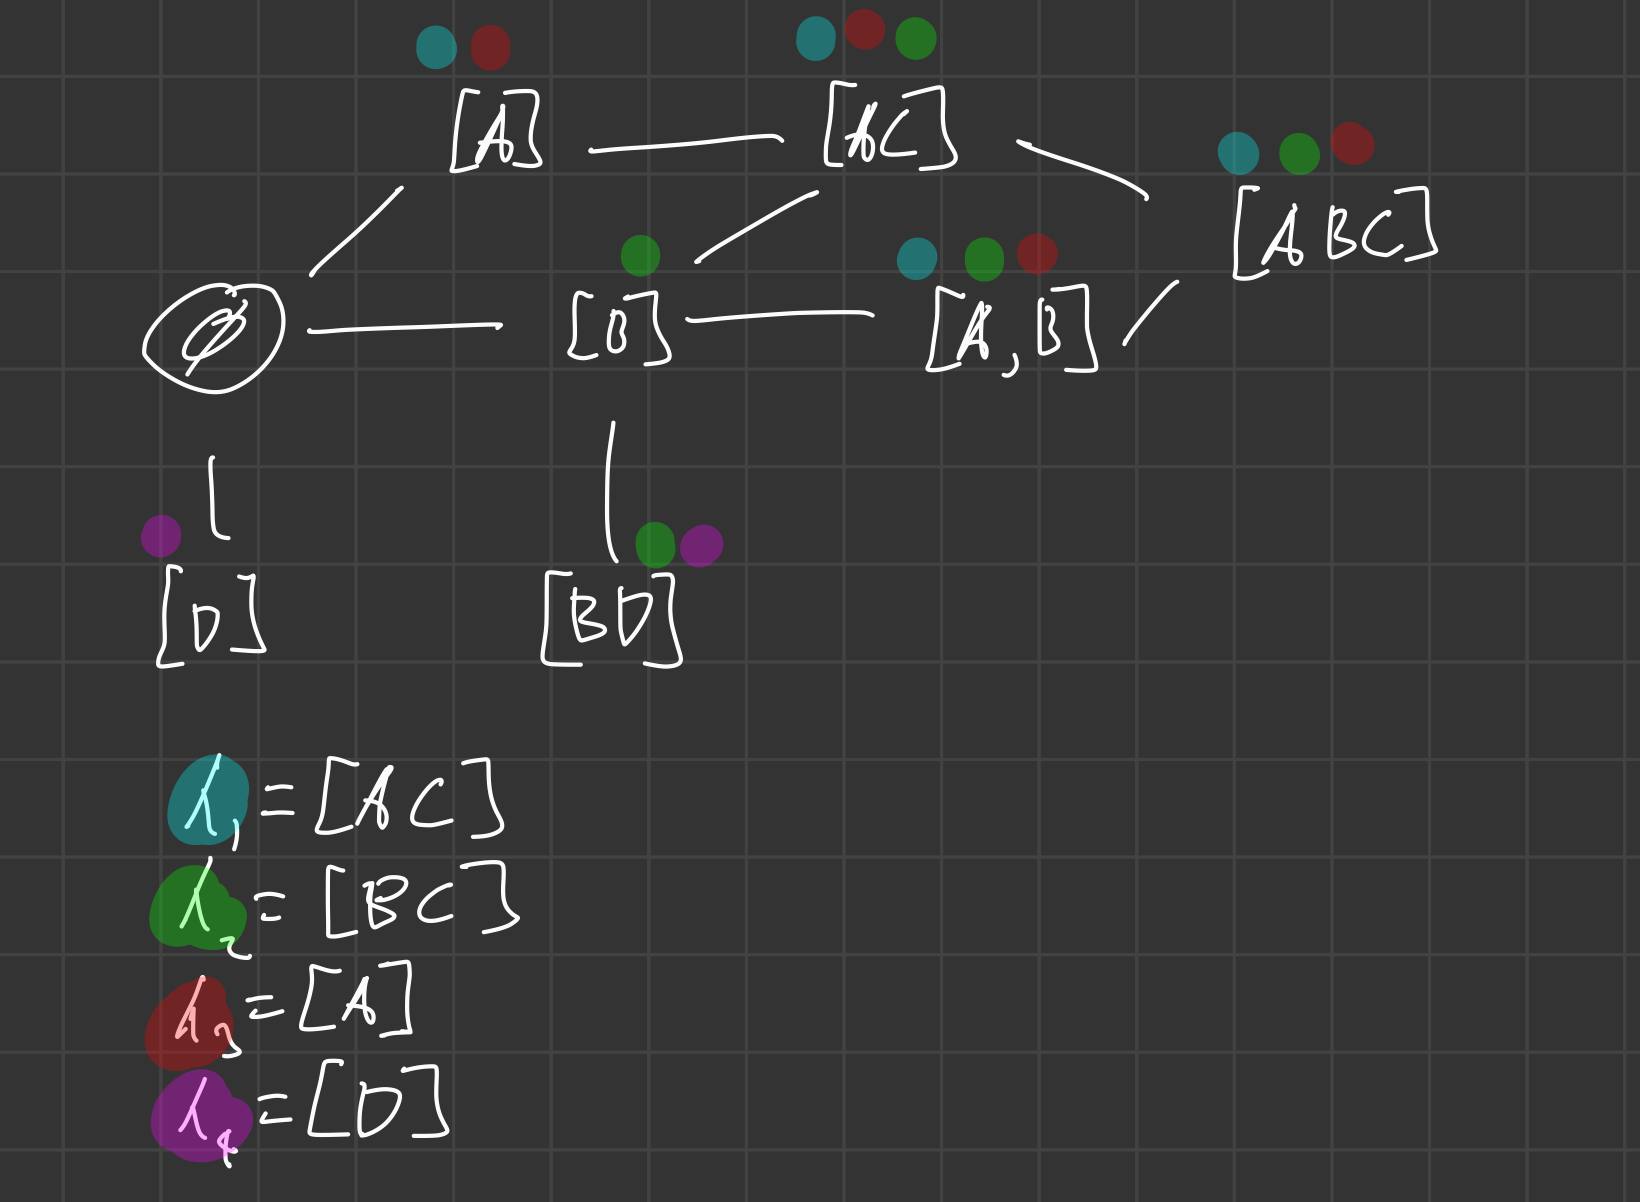
\includegraphics[width=0.8\linewidth]{resources/graph2.png}
    \caption{Example of a Scheduled Entity FSM Graph}
    \label{fig:graph2}
\end{figure}
 
Notice how on any archetype vertex in the graph when there are multiple colors signifies data access contention. Depending on ECS access patterns, an ECS could possibly squeeze a bit more performance but for most cases it is unnecessary. Although, the GECS implementation does provide support for embarrassingly parallel access patterns. So each $\lambda$ may also have some concurrency inside its own function.

\subsection{Entity Consolidation}
A key concept has been omitted thus far is entity consolidation. How, with these systems running concurrently, are entities transitioned between archetypes? It turns out that only entity and component reads/writes are able to be handled in parallel contexts. Component and entity creation/deletion cannot be handled in parallel contexts due to emerging non-determinism on the entity FSM.

The following sections contain a proof made for this paper and a workarounds is suggested.

\subsubsection{Entity Creation/Deletion Operations Leads To Tick Non-determinism}
\label{sec:proof1}
Suppose there exists two systems, systems A and B. Suppose entities live on an entity FSM that contains any set of states and includes some Type C. The purpose of System A is to generate new entities with Type C to place them on the FSM while the purpose of System B is to consume entities with Type C to remove them from the FSM. Both systems A and B run concurrently. 

In such an ECS runtime, entities are generated and transitioned to archetype $\{C\}$. Therefore, the count of entities at archetype $\{C\}$ while the tick is progressing.

There are three cases in which System A and B interact:
\begin{enumerate}
    \item System A generates entities faster than B consumes
    \item System A generates entities at the same rate B consumes
    \item System A generates entities slower than B consumes
\end{enumerate}

Only in case 3 can the next tick occur. The nondeterminism introduced by allowing entity list mutations on the finite state machine can cause program stalls such as in the manner proposed. What this means in a concurrent context is that this can lead to deadlocks, live-locks, or data invalidation.

The same sort of reasoning can be applied to only entity component creation and deletion as well.

\subsubsection{Serializability And Ledger-Based Consolidation}
\label{sec:ledger}
In order to solve the problem of entity consolidation in any context the entity list must stay fixed. That means for each tick, no matter the deletion or additions performed, the entity set must stay the same until the tick is complete. As such, even if perfect concurrent entity consolidation is performed, the effort is wasted. Instead of taking chances at doing concurrent insertions now, why not wait until the serialization point and save the effort? The performance will be the same due to the requirement of the list staying fixed. 

This model proposes to use a ledger-based consolidation technique that caches non-parallelizable operations done on the entity list and applies these operations after the serialization point. The GECS implementation uses separate entity FSM as caches.

\subsubsection{$\delta$ Transition To $\emptyset$}
Since entity deletion causes an entity to transition to $\emptyset$, it is not parallelizable and the fact this entity is deleted must be stored in the ledger. After the serialization point occurs, the ECS will go and clean out all entities that are supposed to translate to the $\emptyset$ directly from the ledger. 

\subsubsection{$\delta$ Transition To Non-$\emptyset$}
Much like the transition to the $\emptyset$, since the entity is transitioning archetypes it is not parallelizable. The transition operation will be stored in the ledger. After the serialization point, then the ECS will perform the $\delta$ transitions. 

\subsection{Model Properties}
The following discusses the two properties that the concurrency model exhibits. Its recursive nature and wait-free-ness. 

\subsubsection{Recursive Design}
\label{sec:recursive_design}
The entity FSM introduced above is only one part of the entire graph generated by an ECS. As stated previously in the definition, an ECS is a set of entity FSM's. 

Consider that each $\lambda$ system given by the user has the signature of $\lambda: W \rightarrow W^\prime$ where each $W^\prime$ represents a modified entity FSM based on $W$. Note that $\lambda$ returns a new structure that contains new entities and only old entities that got moved from their original archetype. This means that $W^\prime$ can represent a ledger of changes to be performed over $W$. It does not matter when these changes are applied to $W$, and there are advantages and disadvantages to processing these ledgers. Chaining these $\lambda$'s will produce a full recursive ECS graph, represented below.

\begin{figure}[htbp]
    \centering
    \begin{verbatim}
                            .     .     .         
                            .     .     .         
                            .     .     .         
                            ^     ^     ^         
                            |     |     |         
                            v     v     v         
                                                
                    ...  <-> W'<-> W <-> W''<-> ...
                                                
                            ^     ^     ^         
                            |     |     |         
                            v     v     v         
                            .     .     .         
                            .     .     .         
                            .     .     .         
    \end{verbatim}
    \caption{ECS graph connected via worlds generated by $\lambda$'s}
\end{figure}

This allows for a graph to naturally build out from $W$ where all edges contain changes to be performed on $W$. Letting a graph build out will in the short run make the engine process ticks faster at the expense of more cache misses later on and shorter vectorization lengths. Concurrency gains are expected to increase the larger the graph of ledgers gets, since simulated archetypes will run on their own thread.

\textbf{Why would this effect the vectorization lengths?} Since different $W$'s are allowed to contain the same archetype, entities over time will slowly be divided between different $W$'s and the original $W$. This means that the composite vector must share the count of entities that contain this typeset over two different vertices, so the lengths are shorter. 

\textbf{Why would this induce cache misses?} In the previous explanation it was discussed how archetype vertices on the FSM must share entities. Suppose this graph contains one system $\lambda$ and it's paired to archetype $A$. Suppose there are 100 entities existing on archetype $A$ before starting. If the graph is allowed to recursively grow for $N$ ticks, and $\lambda$ produces 10 entities, then it would take 10 ticks to produce 200 entities. The entity distribution among the graph looks like below:


\begin{figure}[htbp]
    \centering
    \begin{verbatim}
                        W --> W' --> W'2 --> ... W'10
                        ^     ^       ^           ^  
                        |     |       |           |
                        +---+ +-------+----+------+  
                        |                  |         
                        100          10               
                        Entities     Entities Each    
    \end{verbatim}
    \caption{Entity existing in identical archetypes on ledgers}
\end{figure}

If random access is performed across this set of worlds, cache misses are more likely than if all the entities lived on one archetype, one vector.

\textbf{Why will the concurrency gains increase by processing the ledgers?} Consider the same scenario above used to explain cache misses. Assume that entities all produced by $\lambda$ contain the same archetype signature as $A$, so that each entity is paired with archetype $A$. Using this, suppose it takes 1 second to process 1 entity. This means that $W$ would take 100 seconds and $\{W',\ldots,W^\prime 10\}$ would take 10 seconds each. 

We know that each archetype has its own thread, meaning that in total it would take only 110 seconds to process these entities. If this set of archetypes existing in the ledgers collapsed to $W$, then there would be 200 entities on archetype $A$ an thus take 200 seconds.

GECS does not do this due to thread management concerns and time constraints and spends significant time cleaning the ledger. There is also the concern of query times. For specific systems that exhibit recursive entity generation behaviors, they must be maintained in some manner to prevent the graph from over-growing and slowing down query performance. Due to these concerns, there are special limitations put in place in GECS to prevent recursive ledgers.

\subsubsection{Wait-Free In Model}
The entity FSM introduced in this chapter allows entities to be distributed over a graph and have each archetype perform whatever operations it want's to on this particular archetype without waiting or organizing between other archetypes. 
